\documentclass{article}
\usepackage{graphicx}

\graphicspath{ {images/} }
\begin{document}

\title{%
  Ro-Shan-Bo\\
  \large HW5 - CNS Sapienza}

\author{Giulio Serra 1904089}
\date{December 5, 2019}

\maketitle

\begin{titlepage}
\end{titlepage}

\tableofcontents

\begin{titlepage}
\end{titlepage}

\section{Introduction}\label{sec:intro}
The aim of this documents is to describe the design process of a protocol between two parties to play Ro-Sham-Bo games.

\section{The Ro-Sham-Bo Game}
Ro-Sham-Bo is a simple game consisting of three possible choices (messages): rock, paper or scissors.In order to beat the opponent, the player need to win at least 2p+1 matches choosing between one of the three possible moves, the winner of the match is declared by following these rules: rock beat scissors, scissors beat paper, paper beat rock.

\section{Requirements}
In order to implement an efficient protocol for our game we need to evaluate all the requirements:

\begin{itemize}
 \item \textbf{Matches}\\\\
 	Before beginning a match the two players must decide a number of turns 	to play (2p+1), a player is declared winner if can manage to win at least p+1 games.
	
 	\item \textbf{Messages}\\\\
	During a match they can only exchange three types of messages containing their move(rock, paper or scissors).
	
	\item \textbf{Entities}\\\\
	There are no third parties, servers or trusted authorities, every player must integrally respect the protocol, every player needs to provide informations about her/his choice in the turn. 
	
	\item \textbf{One match at a time}\\\\
	If a player is allready playing a game, cannot begin another one, there must be no way to lie or temper about the outcome of a game/match.

	\end{itemize}
	
\section{Designing the implementation}
Taking into account all the requirements we need to design a protocol where two players can remotely play the Ro-Sham-Bo game, the essential features of our protocol must be: the ability to authenticate the other player before beginning a match, security that a player cannot get unfair advantages while playing(since it will surely exploit it) and the assurance that there is no way to despute about the outcome of a match/game, so starting from the double authentication:

	\begin{figure}[h]
		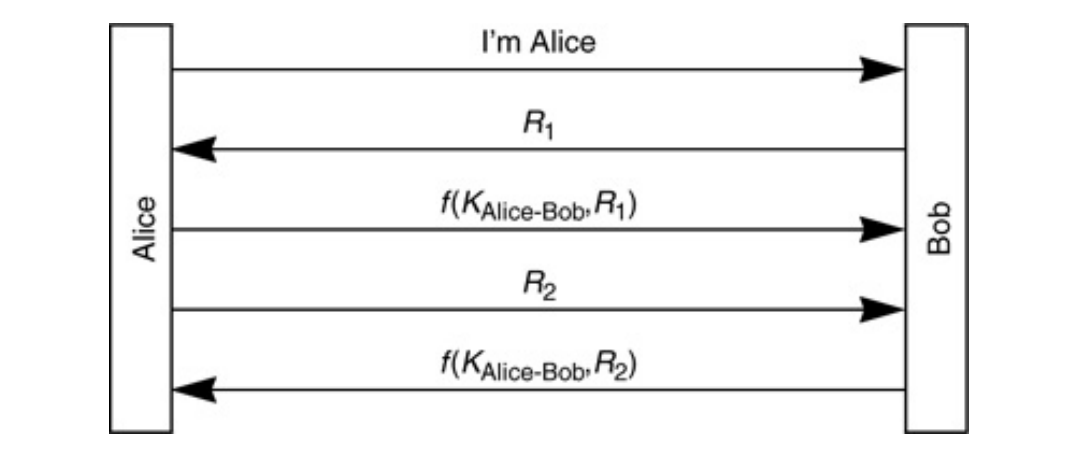
\includegraphics[width=1\textwidth ]{images/doubleAuth.png}
		\centering
	\end{figure}
	
We need to adjust it, in order to meet our requirements, so we need to add a way to: detect if a current session of play is active, a way to exchange messages during a match safely while they cannot be decrypted by the players before the end of the game, and lastly, we need to design a way to implement an agreement to decide wether a player won or loose.

\section{Threat to our protocol}

Starting to design our protocol from the double authentication, expose it to a number of threat:

\subsection{Reflection attack} 
A reflection attack it's a method to comunicate without permissions to a system that uses the same protocol in both directions: basically the attacker tries to make the system reply to it's own challenge.\\The attack consist in: opening a connection to the target, then, when the target tries to authenticate the attacker, he will send a challenge himself to the target and with that response, reply to the first authentication, leaving the second connection opened.\\\\
This type of attacks can be easily avoided, for example, allowing one connection at the time or using different protocols in both directions.

\subsection{Reply attack} 
The reply attack consist in obtaining the informations that an host exchange to another, then send it back pretending to be somebody else.\\
The aim of this attack is not to decrypt informations but rather trying to hide the identity of the attacker in order to get some kind of informations from the host.\\
This type of attacks can be easily avoided by timestamping the data before encryption or by using a token of session.

\section{Implementation}

Here follows a complete implementation for a protocol to support a Ro-Sham-Bo game between two players:

	\begin{figure}[h]
		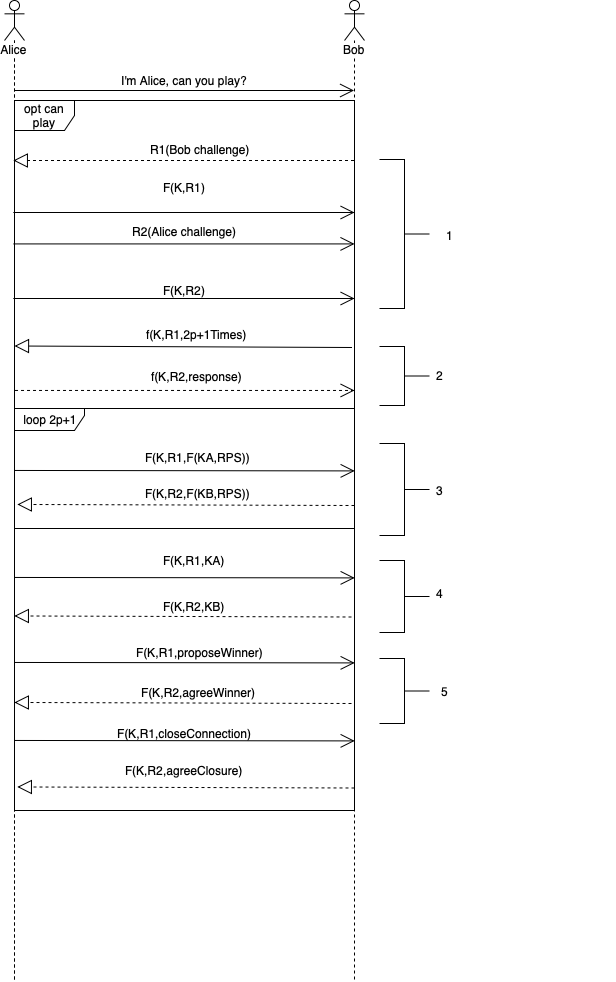
\includegraphics[width=0.7\textwidth ]{images/protocol.png}
		\centering
	\end{figure}
	
The protocol implementation is divided into 6 phases:

\begin{itemize}
 \item \textbf{Phase 1}\\\\
 	In Phase 1 Alice ask to Bob the create a connection , this can be done only if Bob has no open connection to anybody (to prevent reflection attacks).Later Alice create a connection by sharing a key (K) replying 	to Bob's challenge, note that this keys will be use through the whole protocol to exchange messages and authenticate Alice and Bob while exchanging messages between the two. 
 	
	\item \textbf{Phase 2}\\\\
	In this phase the two opponents agree upon the number of turns to declare a winner.
		
	\item \textbf{Phase 3}\\\\
	In these phase each player decide what move to play(rock, paper or scissors), the message is encrypted with a key known only to the player who sent the message, this was done to preventing the player to 	know which move the opponent choose.
	
	\item \textbf{Phase 4}\\\\
	A the end of the turns each player exchange their secret keys to determine a winner.

	\item \textbf{Phase 5}\\\\
	In this phase the two player agree upon a winner, the only way to despute over an outcome to a match/game is straight up lie, because the two players have both their and the other one's moves.
		
	\item \textbf{Phase 6}\\\\
	In this phase the two players close the connection, becoming available for another game.

	\end{itemize}
	
Note that in this configuration, the winner of the game is determined at the end of all the 2p+1 matches, this protocol can be edited to use different keys(one for every match) to immediately declare a winner(like in real life), to do so we need to exchange the secret keys at the end of every match.

\clearpage

\section{References}

	RoShamBo Game:\\
	 \verb|https://en.wiktionary.org/wiki/roshambo|\\
	 \\Reflection attack:\\
	 \verb|https://en.wikipedia.org/wiki/Reflection_attack|\\
	\\Reply attack:\\
	 \verb|https://it.wikipedia.org/wiki/Replay_attack|\\
	
\end{document}